\documentclass[10pt,journal,compsoc]{IEEEtran}
\ifCLASSOPTIONcompsoc
  % IEEE Computer Society needs nocompress option
  % requires cite.sty v4.0 or later (November 2003)
  %\usepackage[nocompress]{cite}
\else
  % normal IEEE
  % \usepackage{cite}
\fi

%\providecommand{\tabularnewline}{\\}

\usepackage{indentfirst}

%%--------------------Colocados por minha vontade própria-----------------------
\usepackage{marvosym}
\usepackage[utf8x]{inputenc} 		
\usepackage[english,brazil]{babel}	
\usepackage[T1]{fontenc}
\usepackage{wasysym}				% setas
\usepackage{picinpar}				% figuras onde eu quero, problemas com referencias
\usepackage{sidecap}				% legenda ao lado da figura
\usepackage[small,bf]{caption}

%\usepackage{fancyhdr}
%\lhead{O que quero no cabeçalho parte esquerda}
%\chead{O que quero no cabeçalho parte central}
%\rhead{O que quero no cabeçalho parte direita}
%\lfoot{O que quero no rodapé parte esquerda}
%\cfoot{O que quero no rodapé parte central}
%\rfoot{O que quero no rodapé parte direita}



%%------------------------------------------------------------------------------
%%----------------Variaveis para o LaTeX no Relatório---------------------------
\newcommand{\hell}{Laborat\'orio de Microprocessadores e Microcontroladores}		%nome do arquivo
\newcommand{\autor}{Luiz, Felipe}							%criador do pdf
\newcommand{\assunto}{Filtro Digital}							%Nome do experimento
\newcommand{\ver}{4$^{\underline{\circ}}$ Experimento - \assunto}						%numeração do experimento
%%------------------------------------------------------------------------------
%%------------------------Detalhes para serem revistos--------------------------
\newcommand{\keyw}{MSP430, Microprocessadores, Microcontroladores, \assunto}	%Keywords
\newcommand{\entrega}{13 de Fevereiro de 2012}				%data de entrega do relatório
%%------------------------------------------------------------------------------
%%------------------------------Nomes-------------------------------------------
%\newcommand{\luiz}{\hyperref[luiz]{Luiz Fernando G. de Oliveira}}
\newcommand{\luiz}{{Luiz Oliveira}}
\newcommand{\luizmatricula}{10/46969}
%\newcommand{\panda}{\hyperref[panda]{Helbert de Oliveira C. Junior}}
\newcommand{\felipe}{{Felipe Carvalhedo}}
\newcommand{\felipematricula}{09/0037791}


%%------------------------------------------------------------------------------
%%	Resolveu o problema de a linguagem não estar declarada
\makeatletter
\def\markboth#1#2{\def\leftmark{\@IEEEcompsoconly{\sffamily}\MakeUppercase{\protect#1}}%
\def\rightmark{\@IEEEcompsoconly{\sffamily}\MakeUppercase{\protect#2}}}
\makeatother
%%------------------------------------------------------------------------------
%%----------------Para inclusão de algoritmos em C/C++/Assembly---------------------------
\usepackage{listings}
%\lstnewenvironment{C}
\lstset{%
language=C,							%linguagem
numbers=left,						%posição dos números
stepnumber=1,						%frequencia de aparição dos números
numbersep=3pt,
tabsize=4,
commentstyle=\color{blue},
basicstyle=\tiny\ttfamily}
% Inclua o source com: \lstinputlisting[language=C]{src/src.c}

\lstdefinelanguage{MSP430}
{ %% Se estiver faltando alguma palavra reservada, insira ela aqui
morekeywords={RRC,SWPB,RRA,SXT,PUSH,CALL,RETI,JNE,JNZ,JEQ,
Z,JNC,JLO,JC,JHS,JN,JGE,JL,JMP,NOP,POP,BR,
RET,CLRC,SETC,CLRZ,SETZ,CLRN,SETN,DINT,EINT,
RLA,RLC,ADD,ADDC,INV,XOR,CLR,MOV,TST,CMP,DEC,
SUB,SUBC,DECD,INC,INCD,SBC,MOV,DADD,BIT,
BIC,BIS,XOR,AND,MOV.B,MOV.W},
sensitive=false,
morecomment=[l]{//},
morecomment=[l]{;},
morecomment=[s]{/*}{*/},
}
% Inclua o source com: \lstinputlisting[language=MSP430]{src/src.asm}


%
%%------------------------------------------------------------------------------
%%---------------------Includes importantes para suporte------------------------
\input link							% Para verificar links de citações e outras configurações
%%------------------------------------------------------------------------------
%%------------------------------------------------------------------------------



% *** GRAPHICS RELATED PACKAGES ***
%

\ifCLASSINFOpdf
  \usepackage[pdftex]{graphicx}  
  \pdfcompresslevel=9
  % declare the path(s) where your graphic files are
  % \graphicspath{{../pdf/}{../jpeg/}}
  % and their extensions so you won't have to specify these with
  % every instance of \includegraphics
  % \DeclareGraphicsExtensions{.pdf,.jpeg,.png}
\else
  \usepackage[dvips]{graphicx}
  % declare the path(s) where your graphic files are
  % \graphicspath{{../eps/}}
  % and their extensions so you won't have to specify these with
  % every instance of \includegraphics
  % \DeclareGraphicsExtensions{.eps}
\fi



% *** ALIGNMENT PACKAGES ***
%
\usepackage{array}
% Frank Mittelbach's and David Carlisle's array.sty patches and improves
% the standard LaTeX2e array and tabular environments to provide better
% appearance and additional user controls. As the default LaTeX2e table
% generation code is lacking to the point of almost being broken with
% respect to the quality of the end results, all users are strongly
% advised to use an enhanced (at the very least that provided by array.sty)
% set of table tools. array.sty is already installed on most systems. The
% latest version and documentation can be obtained at:
% http://www.ctan.org/tex-archive/macros/latex/required/tools/


%\usepackage{mdwmath}
%\usepackage{mdwtab}
% Also highly recommended is Mark Wooding's extremely powerful MDW tools,
% especially mdwmath.sty and mdwtab.sty which are used to format equations
% and tables, respectively. The MDWtools set is already installed on most
% LaTeX systems. The lastest version and documentation is available at:
% http://www.ctan.org/tex-archive/macros/latex/contrib/mdwtools/


% IEEEtran contains the IEEEeqnarray family of commands that can be used to
% generate multiline equations as well as matrices, tables, etc., of high
% quality.


\usepackage{eqparbox}
% Also of notable interest is Scott Pakin's eqparbox package for creating
% (automatically sized) equal width boxes - aka "natural width parboxes".
% Available at:
% http://www.ctan.org/tex-archive/macros/latex/contrib/eqparbox/





% *** SUBFIGURE PACKAGES ***
%\ifCLASSOPTIONcompsoc
\usepackage[tight,normalsize,sf,SF]{subfigure}
%\else
%\usepackage[tight,footnotesize]{subfigure}
%\fi
% subfigure.sty was written by Steven Douglas Cochran. This package makes it
% easy to put subfigures in your figures. e.g., "Figure 1a and 1b". For IEEE
% work, it is a good idea to load it with the tight package option to reduce
% the amount of white space around the subfigures. Computer Society papers
% use a larger font and \sffamily font for their captions, hence the
% additional options needed under compsoc mode. subfigure.sty is already
% installed on most LaTeX systems. The latest version and documentation can
% be obtained at:
% http://www.ctan.org/tex-archive/obsolete/macros/latex/contrib/subfigure/
% subfigure.sty has been superceeded by subfig.sty.




% *** FLOAT PACKAGES ***
%
\usepackage{float}
\usepackage{fixltx2e}
% http://www.ctan.org/tex-archive/macros/latex/base/


%\usepackage{stfloats}
% stfloats.sty was written by Sigitas Tolusis. This package gives LaTeX2e
% the ability to do double column floats at the bottom of the page as well
% as the top. (e.g., "\begin{figure*}[!b]" is not normally possible in
% LaTeX2e). It also provides a command:
%\fnbelowfloat
% to enable the placement of footnotes below bottom floats (the standard
% LaTeX2e kernel puts them above bottom floats). This is an invasive package
% which rewrites many portions of the LaTeX2e float routines. It may not work
% with other packages that modify the LaTeX2e float routines. The latest
% version and documentation can be obtained at:
% http://www.ctan.org/tex-archive/macros/latex/contrib/sttools/
% Documentation is contained in the stfloats.sty comments as well as in the
% presfull.pdf file. Do not use the stfloats baselinefloat ability as IEEE
% does not allow \baselineskip to stretch. Authors submitting work to the
% IEEE should note that IEEE rarely uses double column equations and
% that authors should try to avoid such use. Do not be tempted to use the
% cuted.sty or midfloat.sty packages (also by Sigitas Tolusis) as IEEE does
% not format its papers in such ways.




% *** PDF, URL AND HYPERLINK PACKAGES ***
%
\usepackage{url}
% http://www.ctan.org/tex-archive/macros/latex/contrib/misc/
% 
% \url{my_url_here}.




% *** Do not adjust lengths that control margins, column widths, etc. ***
% *** Do not use packages that alter fonts (such as pslatex).         ***
% There should be no need to do such things with IEEEtran.cls V1.6 and later.
% (Unless specifically asked to do so by the journal or conference you plan
% to submit to, of course. )


% correct bad hyphenation here
\hyphenation{op-tical net-works semi-conduc-tor}

\begin{document}
	\title{
\includegraphics[width=18cm]{./fts/cap.png}\\
	\hell\vspace{1cm}\\\ver\vspace{1cm}}
	\author{
%--------------------------------Nomes------------------------------------------
%		\hyperref[luiz]{Luiz Fernando Gomes de Oliveira},~\IEEEmembership{10/46969} 
%		\\\hyperref[panda]{Helbert de Oliveira Coelho Junior},~\IEEEmembership{10/45253}
\luiz, \felipe\\
\luizmatricula, \felipematricula

		\thanks{Reviewed in \today.}
	}

%--------------------------O titulo é inserido aqui!----------------------------
%	\selectlanguage{english}  %seleciona o idioma em inglês [para mater os termos abstract e o thanks em inglês]
	\markboth{Universidade de Bras\'ilia - Campus Gama - FGA, \entrega}%
%{	\begin{figure*}
%    	\includegraphics[width=\textwidth]{./fts/unb.jpg}
%	\end{figure*}
%}
	{Shell \MakeLowercase{\textit{et al.}}: \ver}
%-------------------------------------------------------------------------------

	\IEEEcompsoctitleabstractindextext{%
	\begin{abstract}
		% objetivo do experimento
% resumo do procedimento (forma como o experimento foi executado)
% os resultados sucintamente discutidos
% Deve ser feito de preferencia em Inglês
%
%
\selectlanguage{brazil}  %%Desta linha em diante coloque o resumo apenas em português. Nas linhas anteriores, mantenha o texto em inglês.
%
Desenvolver um programa que simule um filtro. O filtro é representado pela média das quatro ultimas amostras e assemelha-se a um filtro passa baixa. O resultado do filtro deverá ser expresso em uma barra de LED's, em displays de 7 segmentos ou em um LCD gráfico.
%


	\end{abstract}
	%%-------------------------------------
	\begin{IEEEkeywords} %palavras chaves
		\keyw %,\LaTeX.
	\end{IEEEkeywords}}
	% make the title area
%\onecolumn		%Conferir se pode ser feito em duas colunas

	\maketitle

	\IEEEdisplaynotcompsoctitleabstractindextext
	\IEEEpeerreviewmaketitle

	\selectlanguage{brazil}		%voltando para o português.
	%\tableofcontents			% Sumario

	\section{Procedimentos Experimentais}\label{intro}
		%Definir, caracterizar e mostrar um breve historico e as utilidades do foco



%Segue um exemplo de como INICIAR o texto. Da segunda palavra em
%diante, escreva normalmente
%	\IEEEPARstart{T}{his} demo file is intended to serve as a ``starter file''
%	for IEEE Computer Society journal papers produced under \LaTeX\ using
%	IEEEtran.cls version 1.7 and later.
%
%	\IEEEPARstart{D}{escrição}, com textos e imagens, da configuração do procedimento e cenário experimental. Explorar técnicas e métodos de medida 
%
\subsection{Objetivos}\label{obj}

\IEEEPARstart{E}{ste} experimento tem como objetivo a apresentação de um sinal de onda desconhecido. A apresentação poderá ser efetuada através de uma barra de LED's, displays de 7 segmentos ou com um LCD gráfico. É importante que a apresentação do sinal poderá ser feita de duas formas distintas. A primeira é o sinal exatamente da mesma forma como ele é colhido pelo MSP, a outra opção é utilizando um filtro, que pode ser representado pela equação \ref{filtro}.
	

\subsubsection{Material}\label{mat}
	
\begin{itemize}
	\item MSP430 LaunchPad
	\item Code Composer v4 ou MSPGCC
	\item MSP430G2553
	\item	\begin{itemize}
				\item 10x LED', ou
				\item 4 Displays de 7 segmentos, ou
				\item LCD Gráfico
			\end{itemize}
	\item Protoboard
\end{itemize}	
	
\subsection{Introdução Teórica}\label{intro}
%
%Exemplo de citação: \cite{msp430}
%

Para a realização deste experimento é importante a compreensão de um conversor AD (ADC). O que o conversor analógico/digital faz é capturar amostras do sinal analógico ao longo do tempo.
Cada amostra será convertida em um número, levando em consideração seu nível de tensão. 

\subsubsection{Taxa de Amostragem}\label{tax}

A frequência com que a amostragem irá ocorrer é chamada de taxa de amostragem. Se uma taxa de
amostragem de $22.050 Hz$ for usada, por exemplo, isto significa que em um segundo 22.050 pontos
serão capturados (ou sampleados ). A distância de cada ponto capturado será de $\frac{1}{22.050}$ segundo
(45,35$\mu$s, neste caso). Se a taxa de amostragem for de $44.100 Hz$, isto significa que 44.100 pontos
serão capturados por segundo. Neste caso a distância de cada ponto será de $\frac{1}{44.100}$ segundo ou
22,675$\mu$s, e assim por diante.\cite{cdh}

\subsubsection{Quantização}\label{quant}
Os valores instantâneos da tensão do sinal de entrada, que são obtidos na saída do circuito de amostragem e retenção precisam ser convertidos para a forma digital. Este processo recebe o nome de "quantização".
Os DSPs (Processadores Digitais de Sinais) processam os sinais analógicos convertidos para a forma digital e fazem uso deste processo.
O  que um DSP pode fazer com o sinal vai depender justamente da precisão com que a quantização é feita.
A representação dos valores instantâneos amostrados pelos circuitos anteriores depende do nível de quantização realizado, ou seja, quantos bits são usados para representar cada valor amostrado.
Assim, se usamos 2 bits teremos uma precisão menor do que se usarmos 4 bits para fazer a quantização.

\subsubsection{Resolução}\label{resolucao}

A resolução da conversão indica o número discreto de valores que podem ser produzidos sobre o intervalo de valores analógicos. Os valores são normalmente armazenados eletronicamente de forma binaria, assim a resolução é usualmente expressa em bits. Em consequência, o número de valores discretos disponíveis - níveis - são dados em potência de dois.

A resolução pode também ser definida eletricamente, e expressada em volts. A tensão mínima reconhecida pelo circuito é chamada de bit menos significativo - LSB (\textit{least significant bit}). A resolução (\textbf{Q}) do ADC é igual ao LSB. A voltagem de resolução é dada pela amplitude da tensão dividida pelo número de intervalos de voltagem discretas:

\[
	Q = \frac{E_{FSR}}{N}
\]
	
\begin{SCfigure}[1][h] %%Cuidado..ela não se mantem no lugar
  \centering
  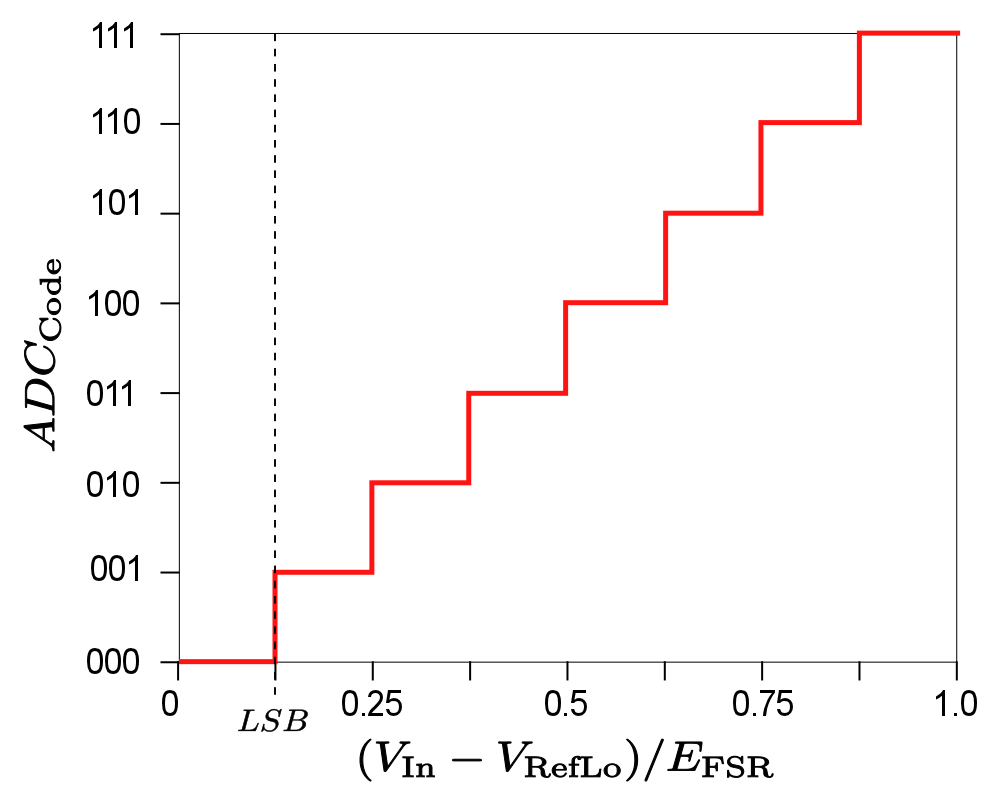
\includegraphics[width=5cm]{./fts/ADC}
  \caption{ Esquema de codificação ADC de 3 bits. Imagem de Wikipedia\cite{wikipedia}}
  \label{caption1}
\end{SCfigure}

Para o experimento, será aplicado um filtro que tem como função cortar as frequências mais altas, mostrando como saída um valor próximo da mediana. Ele pode ser representado pela equação \ref{filtro}, que é a média das quatro ultimas amostras:

\begin{equation}\label{filtro}
	Y=\frac{X_0+X_1+X_2+X_3}{4}
\end{equation}

	
	\section{Descrição do Hardware \& Software}\label{hardsoft}
		% Deve resumir o experimento, os resultados e a discussão (comentários)
% e incluir opiniões do grupo e propostas futuras para o experimento
%Descrição do hardware
%Descrição do software

\subsection{Descrição do Hardware}\label{hardware}

	Pelo grupo ter escolhido apresentar o experimento utilizando apenas o LCD gráfico, modelo LS020, o único circuito eletrônico acrescentado ao LaunchPad foi o LCD e uma bateria de 9V para alimentação do backlight do display, como pode ser observado na figura \ref{f1}.

\begin{SCfigure}[1][h] %%Cuidado..ela não se mantem no lugar
  \centering
  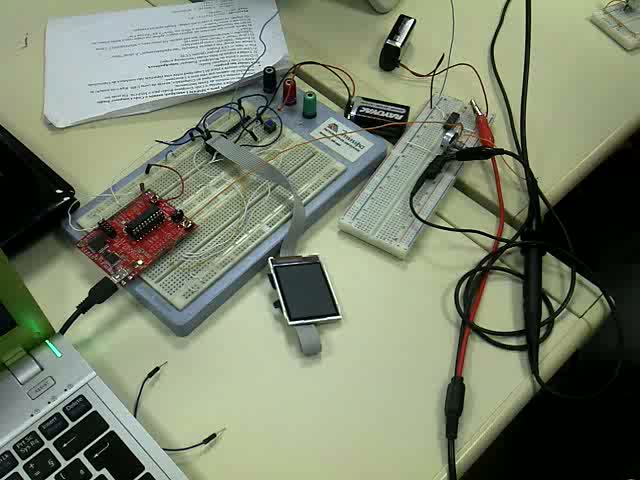
\includegraphics[width=4cm]{./fts/snapshot-001}
  \caption{Vista da protoboard na apresentação final.}
  \label{f1}
\end{SCfigure}



\begin{SCfigure}[1][h] %%Cuidado..ela não se mantem no lugar
  \centering
  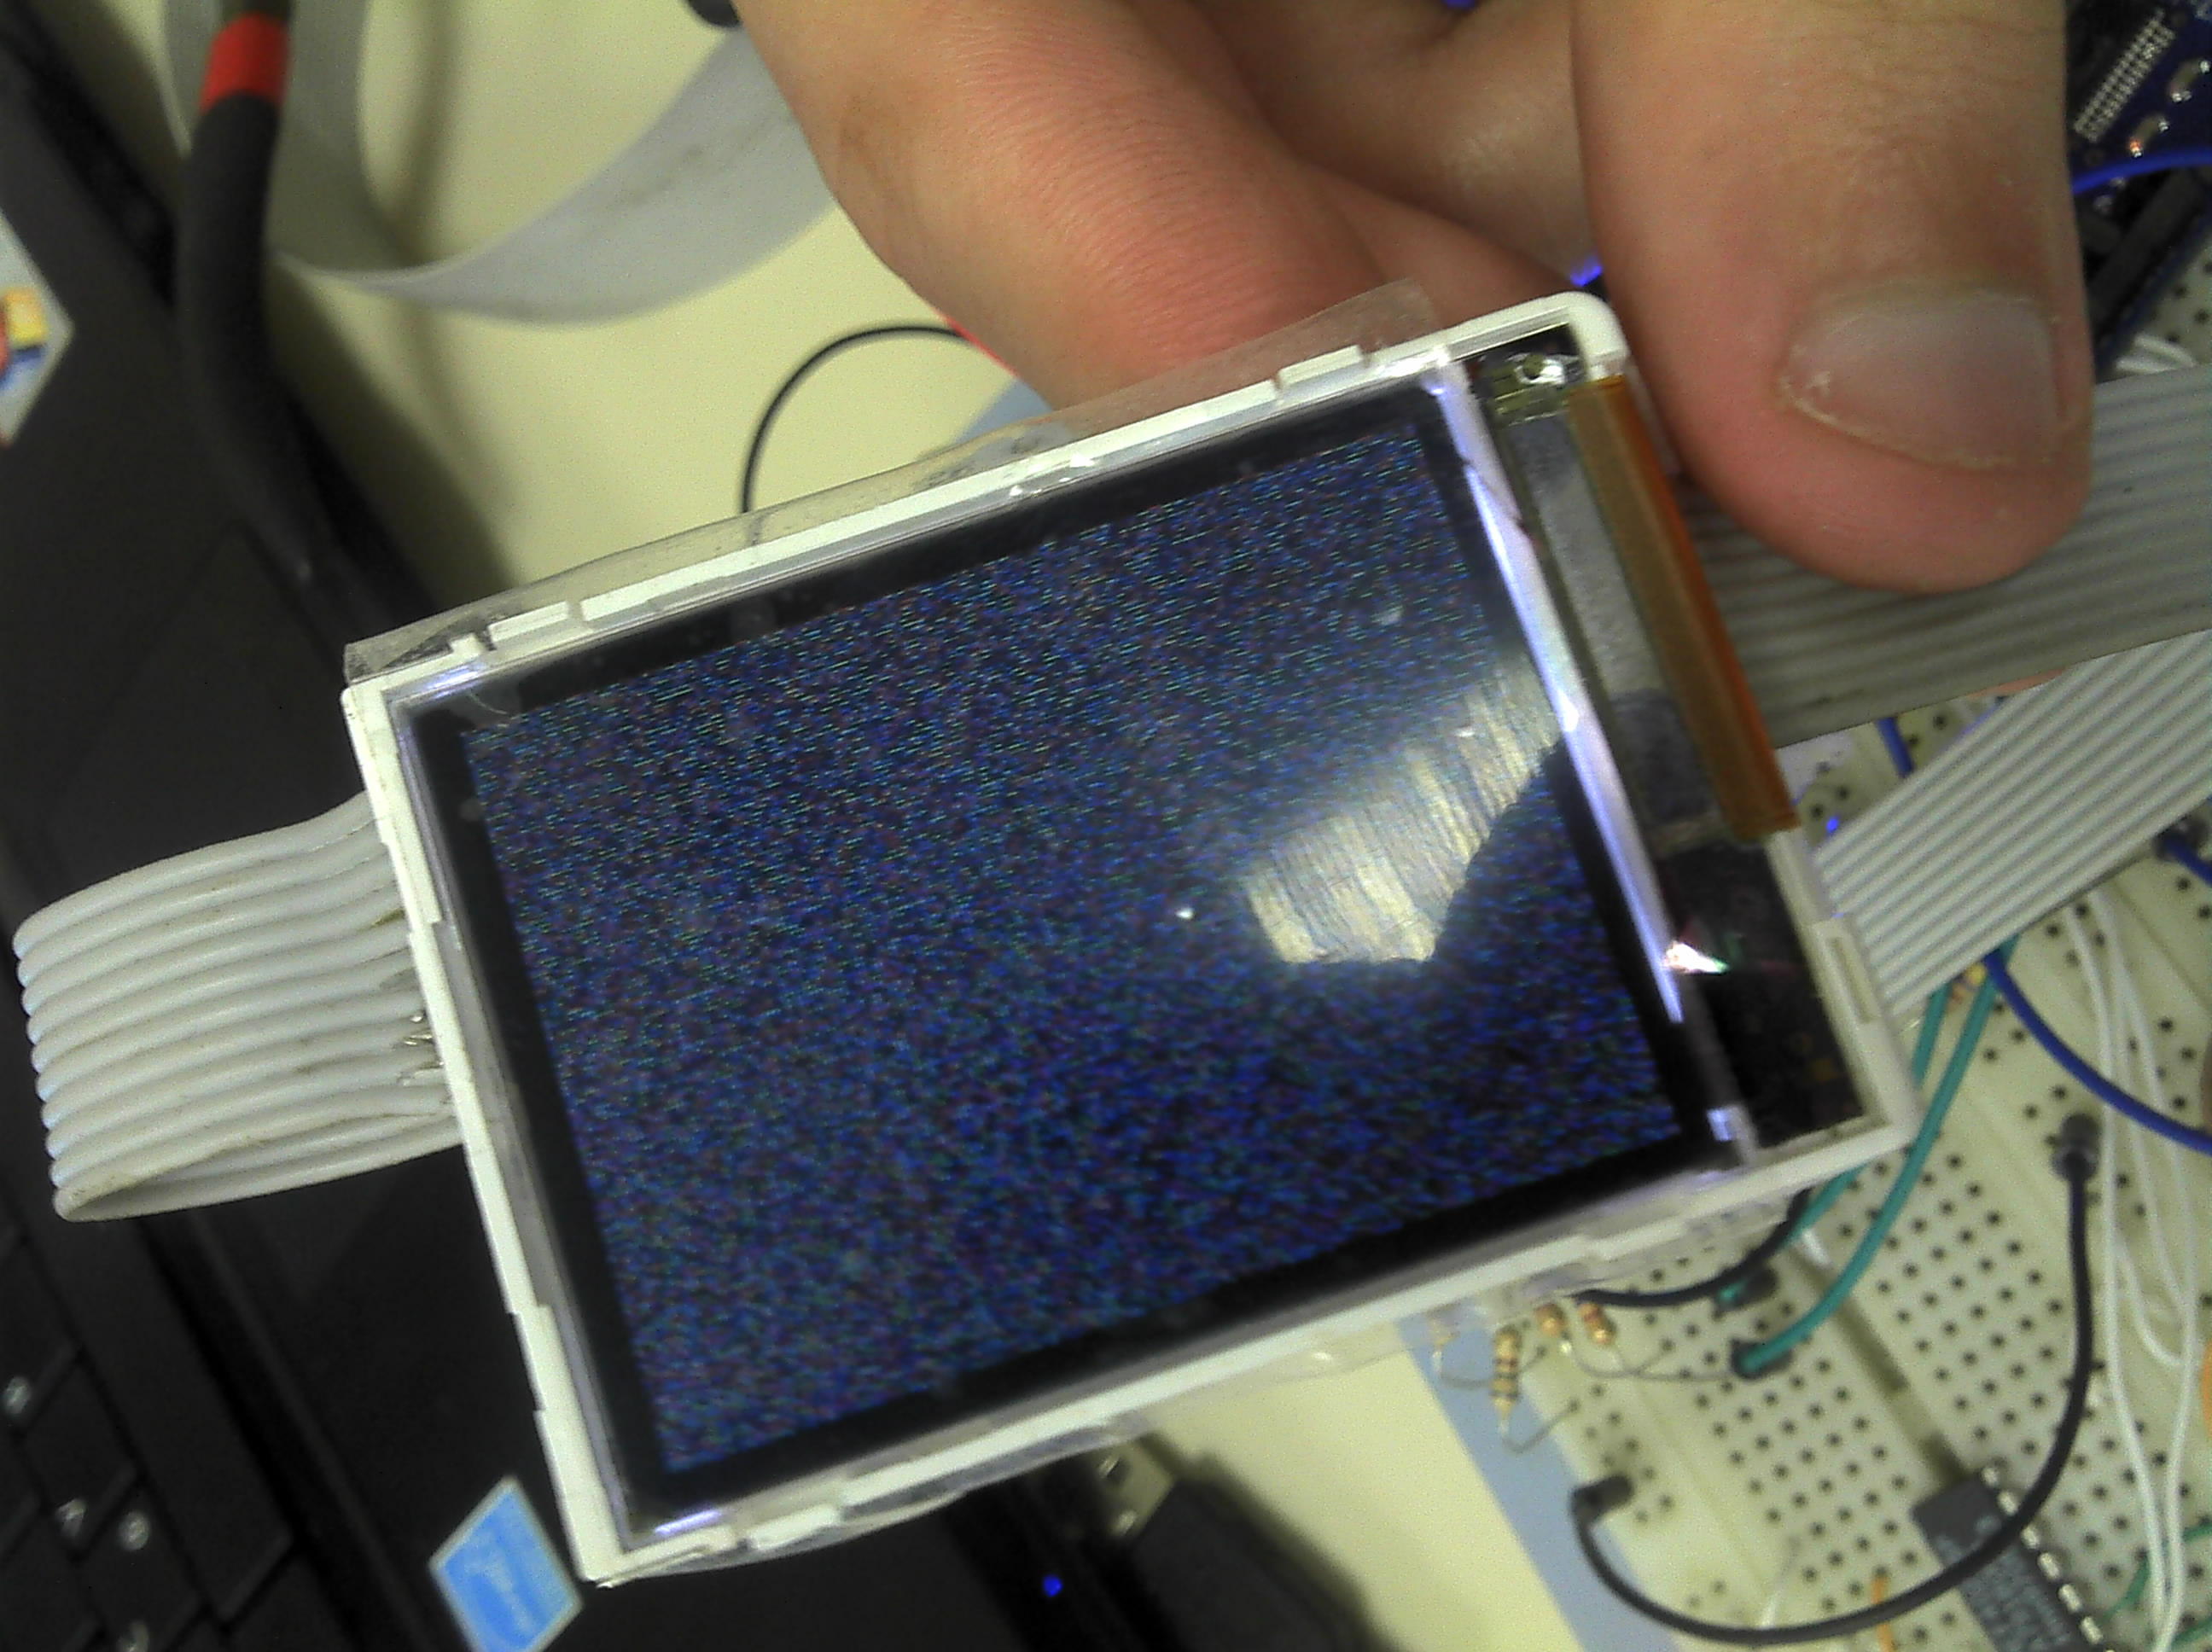
\includegraphics[width=4cm,angle=270]{./fts/f1}
  \caption{Lcd Inicializado.}
  \label{lcd1}
\end{SCfigure}

\subsection{Descrição do Software}\label{software}

Este laboratório teve sem duvidas o código principal mais simples de todos, se desconsiderar todo o código para o funcionamento do LCD. Abaixo encontra-se o arquivo \textit{main.c}, contendo a rotina principal e a interrupção do ADC. Das linhas 11 à 14 o ADC é configurado, habilitado, porém a linha 13 garante que nenhuma amostra será colhida. As linhas 17 e 18 chamas as rotinas para inicializar o LCD (semelhante à figura \ref{lcd1}) e preenche-lo com a cor branca. Em seguida o LED no bit 6 é aceso, representado que o chip esta pronto para inicializar a conversão.

%\lstinputlisting[language=C]{../base.h}
\lstinputlisting[language=C]{../main.c}
%
No laço principal (\textit{while(1)}), a função ploc() é chamada utilizando como parâmetro a variável \textit{ADC10MEM}, que contém o valor atual do ADC. O registrador \textit{ADC10DTC1} é atualizado com 1, para a próxima conversão. Desabilita-se então a interrupção do ADC e espera enquanto o conversor esta ocupado com a conversão. Por fim reconfigura-se o ADC e o coloca em baixo consumo, esperando a próxima colheita. Na interrupção o chip é acordado e é feito um pulso no LED do bit 6. O código teve como  base os exemplos disponibilizados pela Texas Instruments\cite{ti_exemplos}.

\lstinputlisting[language=C]{../ploc.c}

A função ploc é bem simples e apenas plota o valor passado para ela no LCD. Nela é feita a aplicação do filtro, retratado pela equação \ref{filtro}. 

\begin{SCfigure}[1][h] %%Cuidado..ela não se mantem no lugar
  \centering
  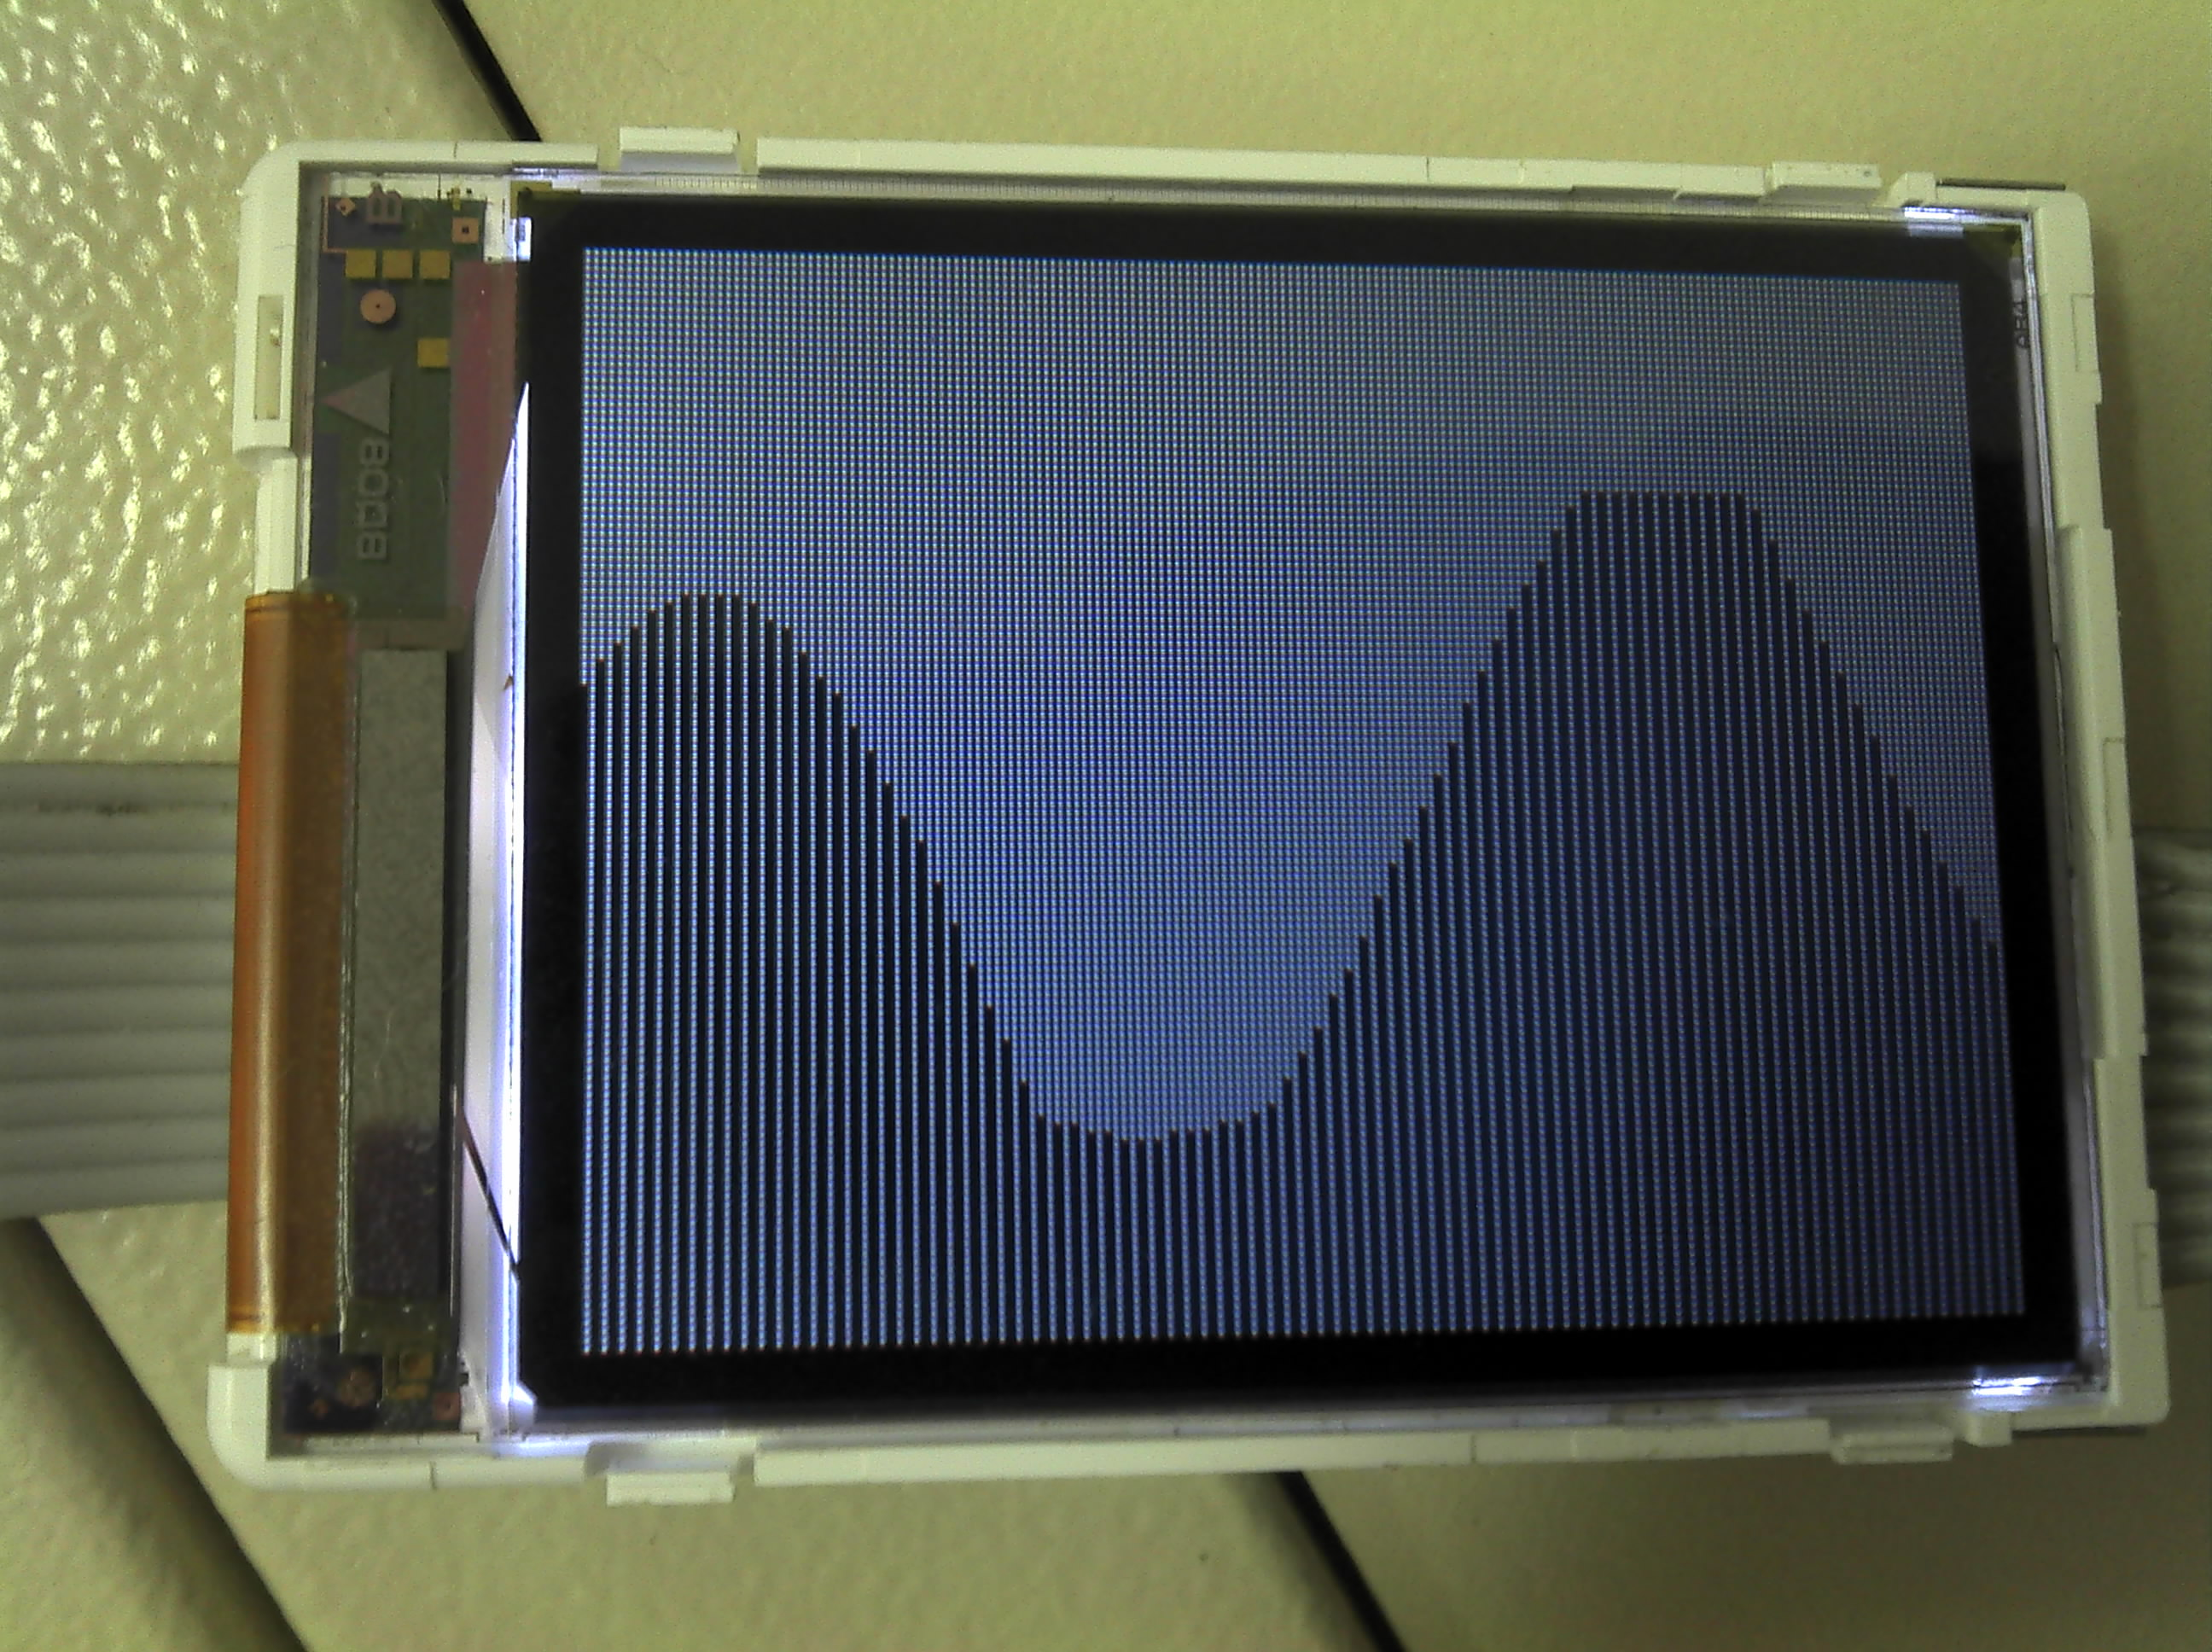
\includegraphics[width=4cm,angle=0]{./fts/snap2}
  \caption{Saída em forma de barras}
  \label{barras}
\end{SCfigure}

Para um maior controle do código, é possivel alterar a saída via código, definindo ou não a macro \textit{\_\_GRAFICO\_BARRAS\_\_} para alterar a saída do display de linhas (figura \ref{linhas}) ou barras (figura \ref{barras}).

\begin{SCfigure}[1][h] %%Cuidado..ela não se mantem no lugar
  \centering
  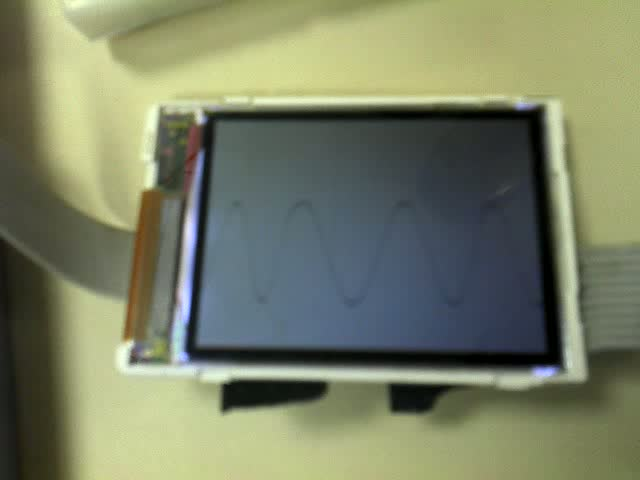
\includegraphics[width=4cm,angle=0]{./fts/snap0}
  \caption{Saída em forma de linhas}
  \label{linhas}
\end{SCfigure}

%\lstinputlisting[language=MSP430]{../prog.asm}

	
	\section{Descrição dos resultados}\label{resultados}
		%Deve conter a tabela verdade obtida em laboratorio comentada
%(principalmente nos estados ambíguos)
%Deve apresentar também as dificuldades encontradas no experimento

%Apresentação dos resultados referentes à confecção do modelo em estudo e medidas realizadas, 
%\begin{SCfigure}[1][h] %%Cuidado..ela não se mantem no lugar
%  \centering
%  \includegraphics[width=4cm]{./fts/unb}
%  \caption{Legenda da figura \ref{caption1}. Coloca qualquer coisa.}
%  \label{caption1}
%\end{SCfigure}
%em forma de texto, tabelas e gráficos, como visto na figura \ref{caption} ou na figura \ref{caption1}. Também pode ser incluida nos anexos, como a figura \ref{unb}.


O grupo conseguiu com este experimento uma grande carga de conhecimento. Não em decorrer da conversão analógico-digital, mas por que fomos responsáveis por levantar a biblioteca do LCD que foi usado especificamente para este experimento. Como observado na função principal, o programa é bem simples, porém o peso da biblioteca do LCD é visível no arquivo final, visto que o executável grava 7378 bytes no MSP, o que é um tamanho bem elevado para apenas uma conversão analógica-digital. 

Outro ponto de grande aprendizado com este experimento foi a reação de filtros e como implementa-los em microcontroladores, visto que foi aplicado no experimento um filtro que tem um comportamento próximo à um filtro passa baixa.


	\ifCLASSOPTIONcaptionsoff
	  \newpage
	\fi

	\bibliographystyle{ieeetr}%{abnt-num}%{ieeetr}%{abnt-alf}
	\bibliography{bibliography}		% expects file "myrefs.bib" 

	%\else
	%\begin{thebibliography}{6} 
	%O Número implica na quantidade MÁXIMA de itens que pode haver de bibliografias.
	%Altere-o se tiver usado mais que duas fontes.

	%\bibitem{IEEEhowto:kopka}
	%H.~Kopka and P.~W. Daly, \emph{A Guide to \LaTeX}, 3rd~ed.\hskip 1em plus
	%  0.5em minus 0.4em\relax Harlow, England: Addison-Wesley, 1999.

	%\bibitem{Wakerly}
	%John F. Wakerly, \emph{Digital Design: Principles and Practices}, 3rd~ed.
	%	\hskip 1em plus 0.5em minus 0.4em\relax Prentice Hall, 1999.

	%\bibitem{zelenovsky}
	%Mendonça A. e Zelenovsky R., \emph{Eletrônica Digital: Curso Prático e Exercícios}, MZ Editora, Brasil, 2004.
	%Contemporary Logic Design - Katz R. H., First Edition, 1993.	

	%\end{thebibliography}
	%\fi

%----------------------Foto e bibliografia do(s) autor(es)----------------------

%	\begin{IEEEbiography}[{\includegraphics[width=1in,height=1.25in,clip,keepaspectratio]{daah_2}}]{Luiz Oliveira}\label{luiz}
%	É, sou eu. Aparecendo aqui só de brinks. Meio que trollando um relatório.
%	\end{IEEEbiography}
%
%	\begin{IEEEbiography}[{\includegraphics[width=1in,height=1.25in,clip,keepaspectratio]{ffuu}}]{Helbert Junior}\label{panda}
%	Pow, eu tinha que aparecer também né?
%	\end{IEEEbiography}
%%------------------------------------------------------------------------------

	\onecolumn
%	\newpage
%	\section{Anexos}\label{anexo}
%		%Inclusão de Anexos
%--------------------Figura logo da UnB----------------------------------------%
%		\begin{figure}[h]
%			\centering
%			\includegraphics [scale=1,angle=0,keepaspectratio=true]{./fts/unb}
%			\caption{Logo da UnB}
%			\label{unb}
%		\end{figure}
%------------------------------------------------------------------------------%		

\cite{ti_exemplos}


		
		
\end{document}


